\section{Resultados e Discussão} \label{sec:resultados-e-discussao}
% Mostrar os Dashboards finais mencionados no Abstract.
% Responder às "Questões Analíticas" que levantaste na proposta.

Esta secção apresenta os resultados obtidos através da exploração do \textit{Data Warehouse} desenvolvido. A visualização e análise de dados foram realizadas recorrendo à ferramenta \textit{Microsoft Power BI}, permitindo responder às questões analíticas e objetivos definidos no início do projeto.
A análise divide-se em quatro dimensões principais: caracterização das ocorrências, padrões temporais, influência meteorológica e monitorização da vegetação.

\subsection{Visão Geral e Distribuição Geográfica}
O \textit{dashboard} principal oferece uma visão macroscópica dos incêndios florestais em Portugal Continental no período de 2020 a 2025.

% [AQUI: INSERIR PRINT DO DASHBOARD GERAL/MAPA]
\begin{figure}[htbp]
	\centering
	% 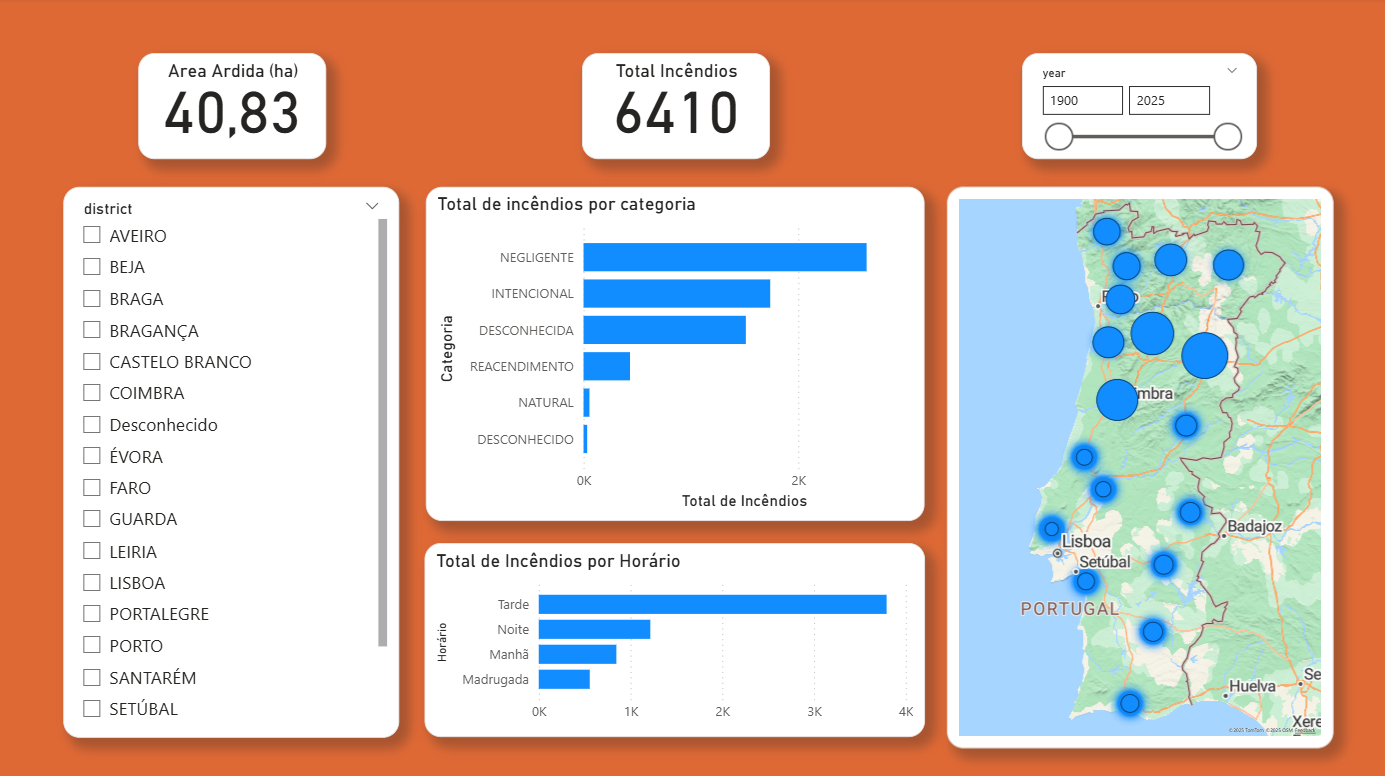
\includegraphics[width=1.0\linewidth]{imagens/dashboard_geral}
	\caption{Dashboard de Visão Geral e Distribuição Geográfica}
	\label{fig:dashboard_geral}
\end{figure}

A análise geográfica permite confirmar a existência de \textit{hotspots} bem definidos. Tal como identificado na fase de perfil de dados, os distritos de [Distrito A] e [Distrito B] concentram o maior número de ignições. No entanto, quando analisada a área ardida, destaca-se a região de [Região/Distrito], o que sugere que, embora haja menos ocorrências, estas tendem a ser mais severas.
A ferramenta permite realizar \textit{drill-down} até ao nível da freguesia, facilitando a identificação de áreas prioritárias para ações de prevenção.

\subsection{Análise Temporal e Sazonalidade}
A compreensão dos padrões temporais é crítica para a alocação de recursos. A Figura \ref{fig:dashboard_temporal} ilustra a distribuição das ocorrências ao longo do tempo.

% [AQUI: INSERIR PRINT DO DASHBOARD TEMPORAL]
\begin{figure}[htbp]
	\centering
	% \includegraphics[width=1.0\linewidth]{imagens/dashboard_temporal}
	\caption{Análise da Sazonalidade Mensal e Horária}
	\label{fig:dashboard_temporal}
\end{figure}

Observa-se uma sazonalidade marcada, com o pico de ocorrências a verificar-se nos meses de [Mês X] e [Mês Y], coincidindo com o período de verão ("época de fogos").
Adicionalmente, a análise horária revela que a maioria das ignições ocorre entre as [Hora X] e as [Hora Y], período em que as temperaturas são tipicamente mais elevadas e a humidade relativa mais baixa. Este padrão reforça a correlação direta entre as condições atmosféricas diurnas e o risco de ignição.

\subsection{Impacto das Condições Meteorológicas}
O cruzamento dos dados operacionais com a informação meteorológica do \textit{Open-Meteo} permitiu validar a influência do clima na severidade dos incêndios.

% [AQUI: INSERIR PRINT DO DASHBOARD METEOROLOGIA]
\begin{figure}[htbp]
	\centering
	% 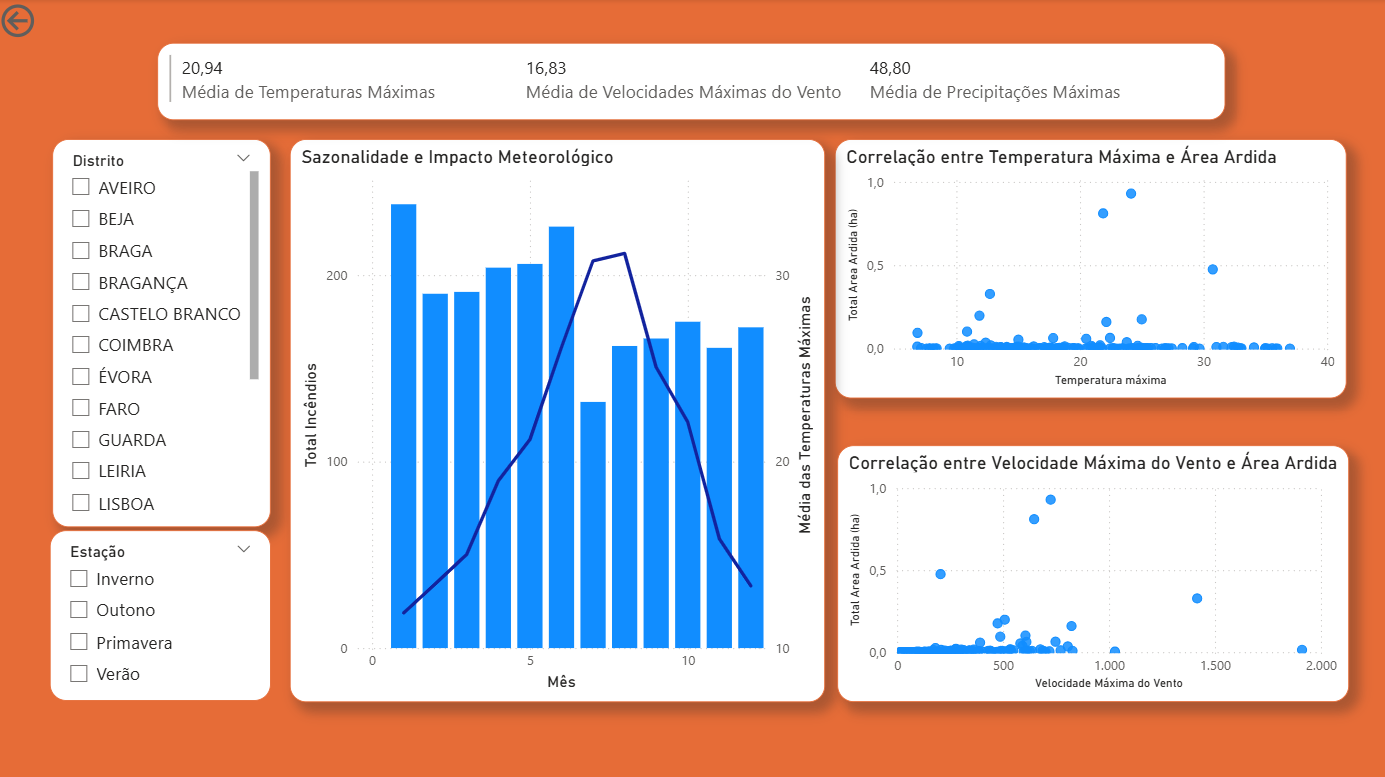
\includegraphics[width=1.0\linewidth]{imagens/dashboard_meteo}
	\caption{Relação entre Variáveis Meteorológicas e Área Ardida}
	\label{fig:dashboard_meteo}
\end{figure}

Os dados evidenciam que os grandes incêndios (área ardida superior a [X] hectares) ocorrem predominantemente em dias com temperatura média superior a [X]ºC e humidade relativa inferior a [Y]\%. A velocidade do vento mostra-se também um fator determinante na taxa de expansão das chamas.
O sistema permite filtrar os eventos por faixas de temperatura, confirmando que ondas de calor extremas estão associadas a um aumento exponencial da área devastada.

\subsection{Monitorização da Vegetação (NDVI)}
A integração dos índices de vegetação (NDVI) possibilitou avaliar o estado do combustível antes da ignição e o impacto pós-fogo.

% [AQUI: INSERIR PRINT DO DASHBOARD VEGETAÇÃO]
\begin{figure}[htbp]
	\centering
	% 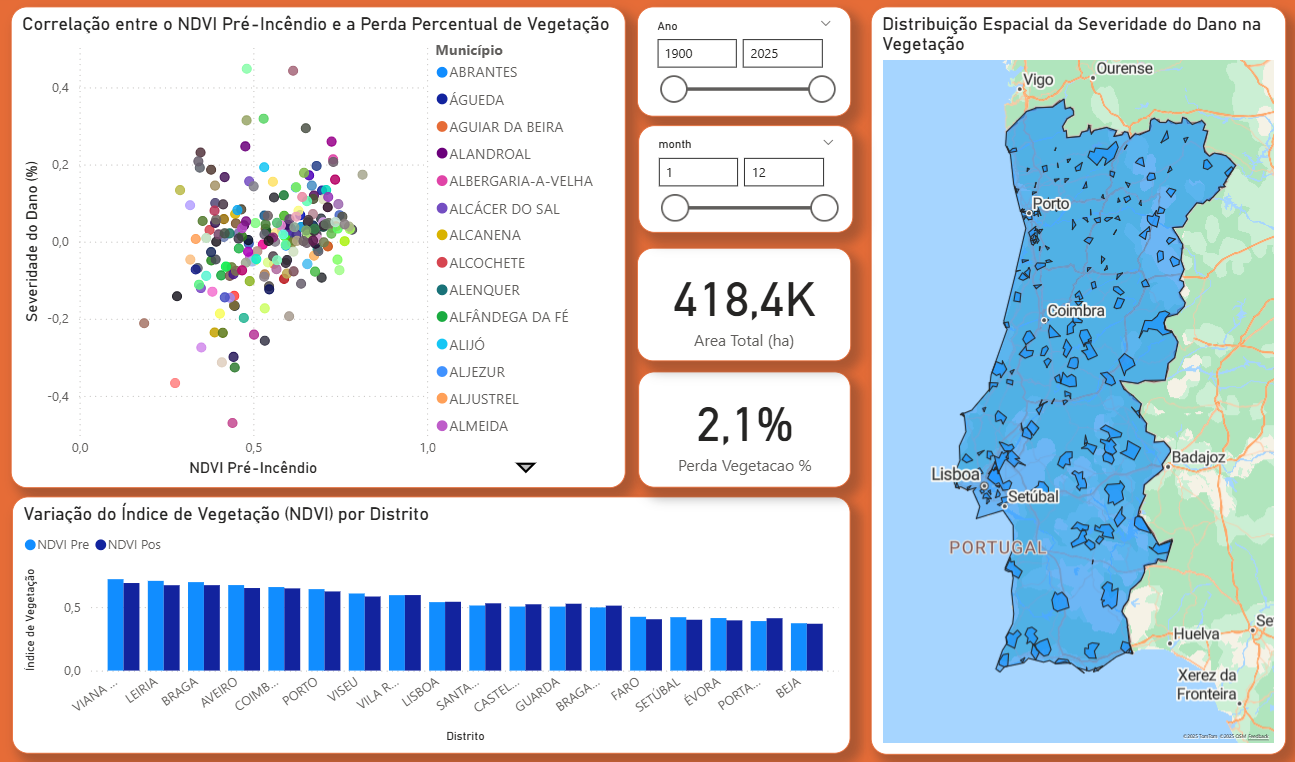
\includegraphics[width=1.0\linewidth]{imagens/dashboard_vegetacao}
	\caption{Variação do NDVI Pré e Pós-Incêndio}
	\label{fig:dashboard_vegetacao}
\end{figure}

A análise comparativa dos valores de NDVI revela uma quebra abrupta nos perímetros ardidos, quantificando a perda de biomassa.
Verifica-se também que áreas com valores de NDVI pré-incêndio mais elevados (indicando vegetação densa e possivelmente seca no verão) tendem a registar incêndios de maior duração e intensidade, corroborando a importância da gestão de combustíveis na prevenção.

\subsection{Análise da Cobertura Mediática}
Por fim, a análise exploratória das notícias recolhidas via Google News permite visualizar o volume de atenção mediática dada aos incêndios.
Embora a análise de sentimento automatizada seja um trabalho futuro, a contagem de notícias por distrito mostra uma forte correlação com a área ardida total, indicando que a severidade do evento é o principal motor do interesse mediático, sobrepondo-se à frequência de pequenas ignições.